\section{Data Acquisition}

Data acquisition from both the FSR sensors and the Shimmer3 devices were set to have a sample frequency of 100Hz. This sample rate was used by others performing similar measurements \cite{Verkerke2005, Byun2016, Sherwani2016}. Additionally, the sample rate were decided to be the same so it was possible to match the two data streams to each other, to enable comparing of measured pressure forces under the feet to movement of the body. A simple graphical user interface (GUI) was developed to match the data. This manual approach were favourable for this project as it was determined that it would be more time consuming to develop an algorithm to automatically match data streams. It would also go beyond the scope for the project.

Data from the Shimmer3 devices was send and saved directly to MATLAB via Bluetooth and stored in $n\times3$ matrices, one for each leg.

For saving acquired data from the FSR sensors, an Arduino program was written to arrange measurements into $n\times6$ matrices. Each column corresponded with the channel input for each FSR. See \figref{fig:FSRNumbering} for the numbering of FSRs and channels. Rows in the matrix were time steps. The data was saved to a $.txt$-file on the microSD card. 

\begin{figure}[H]
	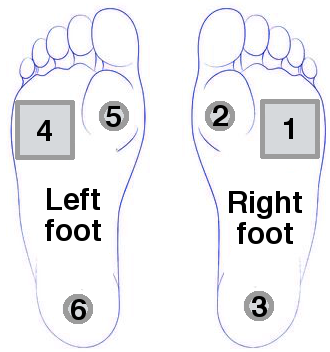
\includegraphics[width=.3\textwidth]{figures/FSRNumbering}
	\caption{The numbering of each FSR sensor according to the channel they were recorded to in the Arduino program.}
	\label{fig:FSRNumbering}  %<--remember LABEL!
\end{figure}



